\documentclass[runningheads]{llncs}

\usepackage[english]{babel}
\usepackage{graphicx}
\usepackage{booktabs}
\usepackage{tabularx}
\usepackage{longtable}
\usepackage{array}
\usepackage{url}
\usepackage{xcolor}
\usepackage{amsmath}
\usepackage[top=1.5cm, bottom=1.5cm, left=1.5cm, right=1.5cm]{geometry}
\usepackage{float}

\newcommand{\FinalClip}{0.886 $\pm$ 0.050}
\newcommand{\FinalLpips}{0.406 $\pm$ 0.092}
\newcommand{\FinalRmse}{0.111 $\pm$ 0.025}
\newcommand{\FinalSsim}{0.761 $\pm$ 0.086}


\newcommand{\modelname}{\texttt{SimianLuo/LCM\_Dreamshaper\_v7}}
\newcommand{\clipmodel}{\texttt{openai/clip-vit-large-patch14}}
\newcommand{\imgpath}[1]{\texttt{#1}}
\setlength{\tabcolsep}{4pt}
\setlength{\textfloatsep}{6pt plus 1pt minus 2pt}
\setlength{\floatsep}{6pt plus 1pt minus 2pt}
\setlength{\intextsep}{6pt plus 1pt minus 2pt}
\setlength{\abovedisplayskip}{4pt plus 1pt minus 2pt}
\setlength{\belowdisplayskip}{4pt plus 1pt minus 2pt}
\sloppy

\begin{document}

\title{Image-to-Prompt Inversion with Structured Prompt Search}
\titlerunning{Image-to-Prompt Inversion}

\author{José Cunha (2021223719) \and Gabriel Pinto (2021220925)}
\authorrunning{José Cunha, Gabriel Pinto}
\institute{University of Coimbra}

\maketitle

\begin{abstract}
This report addresses the image-to-prompt inversion task: given six target images generated with a fixed text-to-image model, recover textual prompts that reproduce them as closely as possible under the same generator, seed, and inference configuration. The final solution treats the problem as discrete prompt optimisation. Candidate prompts are rendered with \modelname, evaluated against the target image with CLIP image-image similarity, LPIPS, RMSE, SSIM, and auxiliary colour/layout metrics, and then ranked. The final submission uses only standard text prompts, fixed LCM inference, and the official seed derived from each filename. Across the final top-3 candidates per target, the mean metrics are CLIP \FinalClip, LPIPS \FinalLpips, RMSE \FinalRmse, and SSIM \FinalSsim.
\keywords{Prompt inversion \and Latent Consistency Models \and CLIP \and LPIPS \and text-to-image generation}
\end{abstract}

\section{Problem and Constraints}

The task consists of recovering prompts for the six target images shown in Fig.~\ref{fig:targets}: \imgpath{1159\_25.png}, \imgpath{1159\_29.png}, \imgpath{1159\_3.png}, \imgpath{1159\_7.png}, \imgpath{7836.png}, and \imgpath{9338.png}. Each prompt is evaluated by rendering it with the same generator setup used for the hidden original image. The seed is the leading number in the filename, for example \imgpath{7836.png} uses seed 7836.

\begin{figure}[t]
  \centering
  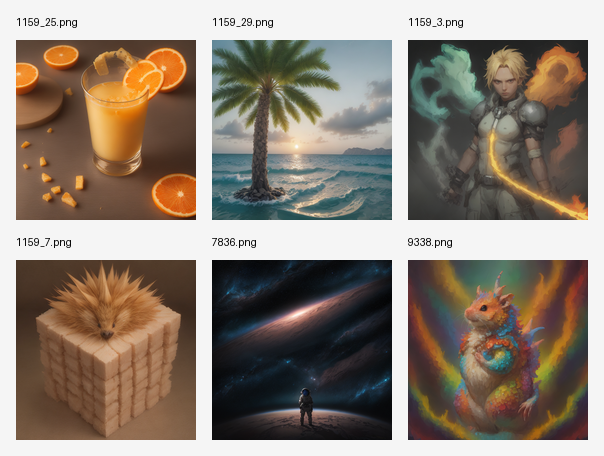
\includegraphics[width=0.50\linewidth]{../imagens/figuras/targets_grid.png}
  \caption{Target images used in the prompt inversion task.}
  \label{fig:targets}
\end{figure}

The final generation configuration is fixed: \modelname, $768\times768$ RGB output, 8 inference steps, guidance scale 8.0, 50 original LCM steps, empty negative prompt, and deterministic seed per target. No ControlNet, LoRA, textual inversion, embedding optimisation, or image conditioning is used in the final render. Those techniques could improve fidelity, but they would change the task from discrete prompt recovery into model or conditioning optimisation.

\section{Methodology}

\subsection{Prompt Search Pipeline}

The project was implemented as an automated prompt search pipeline:
\begin{enumerate}
  \item generate a structured prompt bank for each target;
  \item render each prompt with the fixed LCM configuration;
  \item compute image similarity metrics between target and render;
  \item keep only the best candidates on disk to avoid storage saturation;
  \item refine future prompt banks using the best visual anchors from previous rounds.
\end{enumerate}

The early rounds established semantic anchors using manual prompt engineering, CLIP-guided hard prompt search, PEZ-style discrete token exploration~\cite{pez}, visual anchor extraction, and term ablation. Later rounds moved from broad exploration to targeted refinement: prompts were decomposed into semantic blocks, mutated in controlled combinations, and re-rendered at scale. The last phase focused on the most difficult classes, especially the hedgehog-cube and fantasy hamster, because small wording changes in those targets often caused large structural changes in the render.

\subsection{Experimental History by Round}

The development is presented as 23 experimental rounds. Rounds 1--15 correspond to technical output rounds 24--38, while technical rounds 39--46 are renumbered as rounds 16--23. Additional targeted work performed under technical round 38 is included in round 15. The generator configuration remained fixed, while each round changed how prompts were proposed, rendered, or ranked.

\begin{table}[H]
\centering
\caption{What was performed in each experimental round and what was learned.}
\label{tab:rounds}
\footnotesize
\setlength{\tabcolsep}{2.6pt}
\renewcommand{\arraystretch}{0.82}
\begin{tabularx}{\linewidth}{>{\centering\arraybackslash}p{0.07\linewidth}>{\raggedright\arraybackslash}p{0.50\linewidth}>{\raggedright\arraybackslash}X}
\toprule
Rnd. & Work performed & Result and next decision \\
\midrule
1 & Built manual anchors and expanded subject, background, style, and composition through staged CLIP text--image search. & First usable bank; CLIP also produced visual false positives. \\
2 & Combined semantic-block mutations with PEZ-style optimisation for 1159\_7 and 9338. & Found useful cube and quill vocabulary, but unstable renders. \\
3 & Reused the best renders as visual anchors and generated calibrated block combinations. & Established strong early prompt families. \\
4 & Varied body, material, face, quills/scales, and composition for the two hardest targets. & Five to seven blocks worked better than exhaustive prompts. \\
5 & Re-ranked historical renders with colour, edge, layout, and regional metrics. & Reduced CLIP false positives. \\
6 & Performed term ablation and ordering tests. & Identified indispensable and interfering terms. \\
7 & Sampled factorial combinations of target-specific prompt factors. & Revealed strong interactions between blocks. \\
8 & Added subject, layout, background, and style through a three-level curriculum. & Helped simple targets, not the fantasy creature. \\
9 & Corrected recurring cube, material, belly-colour, and dragon-anatomy failures. & Produced a target-specific failure catalogue. \\
10 & Validated top prompts with the official seed and auxiliary seeds. & Filtered lucky latent coincidences. \\
11 & Compressed prompts and monitored the CLIP token budget. & Confirmed the value of concise diagnostic wording. \\
12 & Added MaxStack regional scores, cross-ablations, and term permutations. & Better detected missing local attributes. \\
13 & Used Codex for 20 VLM-guided refinements on three targets. & No proposal beat its anchor; local refinement was non-smooth. \\
14 & Sampled large English and Chinese block combinations from historical top prompts. & Broad English search dominated and supplied several finalists. \\
15 & Sampled 10\,000 prompts for 1159\_7 and 9338, then added a targeted 9338 repair without dragon/wing terms. & Improved the cube and supplied stronger hamster cues. \\
16 & Searched a 9338 hybrid balancing hamster anatomy, lateral pose, teal belly, scales, and aura. & Improved pose/texture, but no final top-3 image. \\
17 & Blended the strongest targeted-repair and hybrid prompt families for 9338. & Supplied fantasy-hamster ranks 1 and 2. \\
18 & Ran 4\,900 prompts across all targets with five-seed robustness validation. & Supplied warrior ranks 1/3 and astronaut rank 3. \\
19 & Rendered metric-best prompts across 64 seeds per target. & Diagnosed seed sensitivity; non-official seeds were not submitted. \\
20 & Returned to the official fixed seed and changed individual attributes locally. & Supplied orange-juice rank 1 and astronaut rank 2. \\
21 & Applied conservative one-detail-at-a-time prompt variations. & Supplied astronaut rank 1 and fantasy-hamster rank 3. \\
22 & Tested visually proposed changes to liquid, surf, armour, cube structure, and anatomy. & Confirmed useful and harmful local wording changes. \\
23 & Built a minimal-to-detailed prompt ladder for the palm target. & Confirmed that short controlled descriptions were more stable. \\
\bottomrule
\end{tabularx}
\end{table}

The rounds changed role over time. Rounds 1--4 discovered vocabulary and visual anchors; rounds 5--12 improved diagnosis, ranking, and compactness; rounds 13--18 compared VLM repair with increasingly large controlled searches; rounds 19--23 diagnosed seed sensitivity and refined individual attributes under the official fixed seed. The decisive observation was that the generator does not behave like an image editor: a small textual correction can regenerate the whole composition. Consequently, broad sampling around proven anchors, followed by target-specific fixed-seed refinement, was more effective than one iterative correction trajectory.

\subsection{Metrics and Ranking}

Table~\ref{tab:metrics} summarises all measurements used during generation, diagnosis, and final candidate selection. The four primary metrics were available across runs; the auxiliary and target-specific metrics were introduced in later rounds to reject semantic false positives and local structural failures.

\begin{table}[H]
\centering
\caption{Metrics and scores used by the evaluation pipeline.}
\label{tab:metrics}
\footnotesize
\setlength{\tabcolsep}{4pt}
\renewcommand{\arraystretch}{1.04}
\begin{tabularx}{\linewidth}{>{\raggedright\arraybackslash}p{0.25\linewidth}>{\centering\arraybackslash}p{0.10\linewidth}>{\raggedright\arraybackslash}X}
\toprule
Metric / score & Goal & Interpretation and use \\
\midrule
CLIP image similarity~\cite{clip} & $\uparrow$ & Cosine similarity between target and render image embeddings; main semantic-alignment measure. \\
LPIPS AlexNet~\cite{lpips} & $\downarrow$ & Deep perceptual distance; detects differences in texture, local appearance, and object structure. \\
Pixel MSE / RMSE & $\downarrow$ & Mean squared error and its square root on normalised RGB pixels; measures colour and luminance error. \\
SSIM & $\uparrow$ & Structural similarity based on luminance, contrast, and local structure. \\
Colour histogram similarity & $\uparrow$ & RGB histogram intersection; penalises candidates with an incorrect global palette. \\
Edge RMSE / similarity & $\downarrow/\uparrow$ & Distance and derived similarity between Sobel edge maps; evaluates silhouette and internal boundaries. \\
Layout similarity & $\uparrow$ & Agreement of saliency centre, spread, and spatial occupancy; detects misplaced or wrongly scaled subjects. \\
Visual-specific score & $\uparrow$ & Target-dependent combination of diagnostic colour, edge, and spatial properties. \\
Region score & $\uparrow$ & Similarity inside predefined regions of interest, such as cube top/sides or creature belly/body. \\
Heuristic score & $\uparrow$ & Explicit target rules that penalise known failures, including missing regions or separated objects. \\
Saliency components & target-dependent & Number of salient connected components and fraction occupied by the largest one; detects duplication and fragmentation. \\
Normalised metric scores & $\uparrow$ & Per-run normalisation of CLIP, LPIPS, RMSE, SSIM, colour, edge, and layout for combination. \\
Combined / selection score & $\uparrow$ & Weighted aggregate used to rank candidates, with optional Pareto and target-specific bonuses. \\
\bottomrule
\end{tabularx}
\end{table}

The metrics are complementary: CLIP can rank semantically plausible but visually wrong images too highly, while pixel metrics can favour a compatible background despite an incorrect subject. The final ranking is therefore metric-based but never relies on one measurement alone. For cross-run comparison, candidates were also re-scored with the raw metric average:
\[
\frac{\mathrm{CLIP} + (1-\mathrm{LPIPS}) + (1-\mathrm{RMSE}) + \mathrm{SSIM}}{4}.
\]
The result tables expose the four comparable raw metrics rather than only the internal selection score.

\subsection{Implementation}

Rendering and evaluation were implemented in Python. The main scripts are \texttt{search\_streaming\_topk.py}, \texttt{search\_multiseed\_validate.py}, and \texttt{search\_seed\_sweep.py}. The streaming design renders candidates one by one, evaluates them immediately, and stores only the top-k images and CSV metrics. This was necessary because several rounds generated thousands of candidates per target and storing every render would exceed the available disk space.

The final prompt bank combines the strongest historical anchors, small targeted variants, and multi-seed validation used only to discover robust prompt families. The submitted renders remain fixed-seed renders, as required by the task.

\subsection{Experimental Setup and Reproducibility}

All final candidates were rendered from text only. The target image is used exclusively by the evaluator, never by the generator. This distinction is important because the task is not image reconstruction with conditioning; it is prompt recovery under a deterministic generation environment. The render seed is read from the filename and the same prompt can therefore be re-rendered independently by another user if the model checkpoint and scheduler configuration are available.

The experiments were organised as timestamped output folders. Each run stores a prompt bank, the retained top-k images, and a CSV file with the raw metrics and the internal ranking score. This makes the search auditable: if a later prompt looks visually better but receives a worse metric score, both the image and its score remain available for inspection. The final report was generated from the consolidated top-3 CSV, not by manually copying isolated values into the text.

\begin{table}[t]
\centering
\caption{Reproducibility-relevant pipeline configuration.}
\label{tab:repro}
\footnotesize
\setlength{\tabcolsep}{10pt}
\begin{tabular}{ll}
\toprule
Component & Value / rule \\
\midrule
Model and resolution & \modelname, $768\times768$ RGB \\
Seed rule & leading numeric prefix of target filename \\
Scheduler & LCM, 8 inference steps, 50 original steps \\
Guidance and negative prompt & CFG scale 8.0, empty negative prompt \\
Storage & streaming top-$k$ retention \\
Primary metrics & CLIP, LPIPS AlexNet, RMSE, SSIM \\
Auxiliary metrics & colour histogram, Sobel edge, layout/regional scores \\
\bottomrule
\end{tabular}
\end{table}

The notebook and scripts were used differently during development. The notebook is useful for interactive inspection, small runs, and visual comparison. The scripts are more reliable for long searches because they stream progress, write metrics incrementally, and can be restarted with a smaller prompt bank if disk space becomes a constraint. This separation reduced the risk of losing a long run and made the final results easier to reproduce.

\subsection{Computational Budget and Storage Management}

The search was constrained by both GPU time and disk usage. Rendering a single LCM image is relatively fast compared with standard diffusion sampling, but thousands of prompts across six targets still produce long runs. The early experiments saved many intermediate images, which quickly became impractical. The later scripts therefore changed the workflow: candidate images were rendered, scored, and discarded unless they entered the current top-k list for their target.

This streaming strategy changed how experiments were planned. Instead of launching one very large blind run, prompt banks were divided into focused rounds. A broad round was used to discover promising families; later rounds reused only the strongest families and explored smaller local mutations. This reduced wasted rendering and made it possible to inspect results between rounds without filling the disk with low-ranking candidates.

The multi-seed runs were also treated carefully. Rendering the same prompt under many seed offsets is useful for discovery, but it multiplies cost quickly. For this reason, seed sweeps were applied only to a small number of metric-best prompts or to classes where the visual identity was unstable. The final render remained fixed-seed, so the extra seeds were an analysis tool rather than part of the submitted output.

From a practical perspective, this matters because prompt inversion rewards iteration. A technically elegant search method that cannot be run repeatedly is less useful than a simpler streaming pipeline that can be inspected, cleaned, and resumed. The final workflow prioritised this robustness: every important run produced CSV metrics, a small set of images, and enough metadata to trace each result back to the prompt that generated it.

\subsection{Prompt Design Principles}

Prompt length was controlled because the text encoder has a limited effective context, commonly around 77 CLIP tokens. Long prompts were not simply truncated problems; they also created concept competition. If a prompt for the warrior simultaneously mentions \emph{silver armour}, \emph{golden sword}, \emph{fire}, \emph{mist}, \emph{reflection}, \emph{anime}, \emph{mage}, and \emph{low contrast}, the model may satisfy the words globally but not preserve the target composition. The final prompts therefore keep the number of semantic blocks small and place the most important concept first.

The prompt templates were structured as object identity, geometry or material, discriminative colour, layout, background, and style. Terms were removed when they repeatedly caused harmful side effects. For instance, \emph{dragon} helped explain the fantasy creature scales but often produced wings and reptile anatomy; \emph{creaminess} helped the orange juice opacity but could make the liquid too milky; \emph{surf} helped the palm image but easily created waves that were too high. Table~\ref{tab:promptdesign} summarises the final target-specific design choices.

\begin{table}[t]
\centering
\caption{Prompt design decisions by target.}
\label{tab:promptdesign}
\resizebox{\linewidth}{!}{%
\begin{tabular}{p{0.15\linewidth}p{0.33\linewidth}p{0.23\linewidth}p{0.21\linewidth}}
\toprule
Target & Stable visual blocks & Harmful or unstable wording & Remaining limitation \\
\midrule
1159\_25 & clear glass, pale orange juice, orange slice, brown studio surface & too much ``creamy'', too many garnish details & exact foam and slice geometry \\
1159\_29 & single slender palm, shallow turquoise ocean, gentle surf, low sun reflection & strong surf, beach, island, dramatic sunset & trunk position and cloud shadow \\
1159\_3 & blond anime warrior, pale/silver armour, orange energy, blue-green mist & highly reflective armour, too many weapon terms & pose and blade path instability \\
1159\_7 & wooden cube body, peach tile sides, hidden muzzle, radial orange quills & normal hedgehog, basket, waffle, toy box & exact 5x5x5 block separation \\
7836 & tiny astronaut, curved ground arc, diagonal pale pink stripe, blue nebula haze & edge-only nebula, large astronaut, bright planet & stripe location and horizon curvature \\
9338 & hamster anatomy, orange snout, teal belly patch, rainbow scale quills, painterly aura & full dragon, wings, generic cute animal & hybrid anatomy and body texture \\
\bottomrule
\end{tabular}%
}
\end{table}

\subsection{Concrete Prompt Refinement Examples}

Several improvements came from replacing broad descriptions with model-sensitive wording. Table~\ref{tab:examples} shows representative refinements that were useful during the final rounds. These examples are not meant to list every tested prompt, but to illustrate the type of reasoning used when moving from a caption-like description to a prompt that better controls the LCM.

\begin{table}[H]
\centering
\caption{Examples of prompt refinements used during the search.}
\label{tab:examples}
\footnotesize
\begin{tabular}{p{0.16\linewidth}p{0.35\linewidth}p{0.39\linewidth}}
\toprule
Target & Less effective wording & More effective wording or decision \\
\midrule
Orange juice & creamy orange drink, detailed garnish, many fruit pieces & pale orange juice, single clear glass, minimal citrus pieces \\
Palm tree & beach sunset with waves and island background & single slender palm tree rising from shallow turquoise ocean \\
Warrior & reflective silver armour, dramatic glowing weapon & pale/silver armour, low contrast, controlled orange energy \\
Hedgehog-cube & cute hedgehog in a wooden box & small hedgehog in wooden cube, peach tile sides, muzzle hidden \\
Astronaut & astronaut near nebula at the edge of space & tiny astronaut bottom center, diagonal pale pink planetary stripe \\
Fantasy hamster & rainbow dragon hamster with fantasy scales & hamster anatomy, teal belly patch, scale quills only on back/shoulder \\
\bottomrule
\end{tabular}
\end{table}

The examples show two recurring principles. First, the most important object should appear early and in a compact form. This reduces the chance that the model creates a different central subject. Second, modifiers should be discriminative rather than decorative. Words such as \emph{dramatic}, \emph{fantasy}, or \emph{glowing} can improve style, but they are dangerous when the target requires precise geometry. In the final prompt banks, these words were either removed or placed after the structural terms.

The refinements also show why failed prompts were still useful. When a word consistently caused a visible failure, it became a negative clue for later manual design. For example, \emph{beach} usually introduced land into the palm scene, \emph{dragon} often produced wings or reptile anatomy in the hamster target, and \emph{reflective} made the warrior armour too shiny. Removing these terms was often more effective than adding new ones.

\subsection{Round-to-Round Decision Rules}

The prompt banks were not expanded uniformly. After each run, the next round was selected according to the type of error observed in the best candidates. If the target identity was wrong, the next bank changed the first noun phrase and reduced style terms. If the identity was correct but the layout was wrong, the next bank changed spatial wording such as \emph{bottom center}, \emph{diagonal stripe}, \emph{single slender tree}, or \emph{foreground water}. If colour was the main error, the next bank changed only the palette terms and kept the object phrase fixed.

This rule prevented unnecessary search. For example, once the orange juice consistently produced a single glass, later variants focused on liquid opacity, garnish quantity, and table fragments rather than trying new photographic styles. Once the astronaut consistently appeared at the bottom of the image, later variants focused on the diagonal pink stripe and blue haze. In contrast, the fantasy hamster required repeated identity-level changes because many high-scoring renders still drifted toward a dragon or generic mascot.

The same logic was used to decide when to stop a class. A class was considered locally saturated when new prompt variants improved one metric but degraded the visual match or another important metric. At that point, rendering more variants from the same wording family was less useful than moving budget to a weaker target. This is why the final search concentrated on the warrior, hedgehog-cube, and fantasy hamster after the orange juice, palm tree, and astronaut had reached stable prompt families.

\subsection{Metric Interpretation}

The best candidate per target should not be read as a single absolute quality number. A high CLIP value means that the main semantic class is present, but it does not guarantee the correct layout. For example, the fantasy hamster obtains a strong CLIP score because the rendered creature contains animal, colour, and fantasy cues, yet its LPIPS and SSIM remain weaker because the exact hybrid anatomy is not stable. Conversely, the hedgehog-cube has a lower CLIP score than the orange juice but very strong RMSE and SSIM because the object occupies a compact region on a simple background.

The orange juice and palm tree are the most semantically straightforward targets. Their prompts describe familiar photographic scenes and the generator has many plausible examples of these concepts. The astronaut is also stable because the composition is dominated by background colour and a diagonal light band; the small human figure contributes less to pixel error than it would in a close-up portrait. The warrior and fantasy hamster are harder because small prompt changes alter the subject itself: facial expression, armour, blade geometry, scale placement, and body proportions all vary together.

The reported top-3 candidates are therefore intended to show robustness rather than only the single best render. In some classes, the first candidate is clearly strongest across most metrics; in others, rank 2 or rank 3 may be visually preferable for a particular detail. This is expected in prompt inversion: the ranking score approximates visual similarity, but exact human preference can depend on which target attribute is considered most important.

\subsection{Target-Specific Evaluation Priorities}

Although the same core metrics were computed for every image, each target required a different interpretation of those metrics. For \imgpath{1159\_25.png}, colour fidelity and product-photography realism were more important than strict edge matching, because small changes in fruit fragments do not alter the main identity of the image. For \imgpath{1159\_29.png}, layout and colour were both important: a render could contain a correct palm tree but fail if the horizon, water reflection, or wave scale changed too much.

For \imgpath{1159\_3.png}, semantic correctness was not enough. CLIP could identify an anime warrior even when the blade, armour shine, or fire/mist balance were wrong. This made LPIPS and visual inspection especially useful. For \imgpath{1159\_7.png}, the cube silhouette and block-like material were decisive, so pixel-level structure, edge similarity, and SSIM were more informative than object-class semantics alone. For \imgpath{7836.png}, RMSE and SSIM were strong indicators because the image is dominated by dark sky, a diagonal luminous stripe, and a small bottom figure. For \imgpath{9338.png}, the challenge was hybrid identity: the model had to preserve hamster anatomy while adding scale quills and a colourful aura, so no single metric was sufficient.

This target-specific interpretation also guided prompt generation. Simple scenes benefited from conservative wording, while hybrid or stylised scenes needed more discriminative terms. The evaluation pipeline therefore used the same base measurements for all targets, but the analysis of failures and future prompt variants was always class-specific.

\subsection{Final Selection Policy}

The final selection policy combined automatic ranking with conservative manual validation. Automatic ranking determined the candidate order, but candidates were visually checked to reject obvious artefacts that metrics sometimes miss, such as duplicated subjects, unrelated objects, or a completely wrong central figure. No candidate was promoted only because it looked subjectively pleasant; visual inspection was used as a guardrail against metric failures, not as a replacement for the metric score.

The top-3 format is useful because prompt inversion is inherently uncertain. A single best prompt can overfit the metric stack, while a ranked set shows whether the search found a stable prompt family. For the orange juice, the top prompts are close variations of the same product-photo structure, which indicates convergence. For the palm tree, the top prompts share the ocean and single-tree layout but trade off water activity and cloud appearance. For the warrior, the top prompts reveal the instability of energy placement and armour reflectance. For the hedgehog-cube, all strong candidates preserve the cube body and quill cap, showing that the structural prompt family is robust. For the astronaut, variations mostly affect stripe position and nebula density. For the fantasy hamster, the top-3 candidates expose the main trade-off between hamster anatomy and scale/quill detail.

This policy also avoids overclaiming. Some final images are clearly better than earlier runs, but the task is not solved perfectly. The report therefore presents the best measurable candidates together with their limitations. This is preferable to reporting only the most visually appealing image, because it keeps the final result reproducible and connected to the evaluation pipeline.

\section{Results}

Figure~\ref{fig:finaltop3} shows the target image and the three selected reconstructions for each target. Table~\ref{tab:top3} reports the comparable ranking score, metric values, and source output round for all final top-3 candidates. Before fixing this figure and table, all round-level CSV files with recoverable fixed-seed renders were scanned and compared with the curated final CSV; the selected set remained the strongest valid fixed-seed set, especially for the hedgehog-cube where raw round scans missed stronger archived finalists.

\begin{figure}[p]
  \centering
  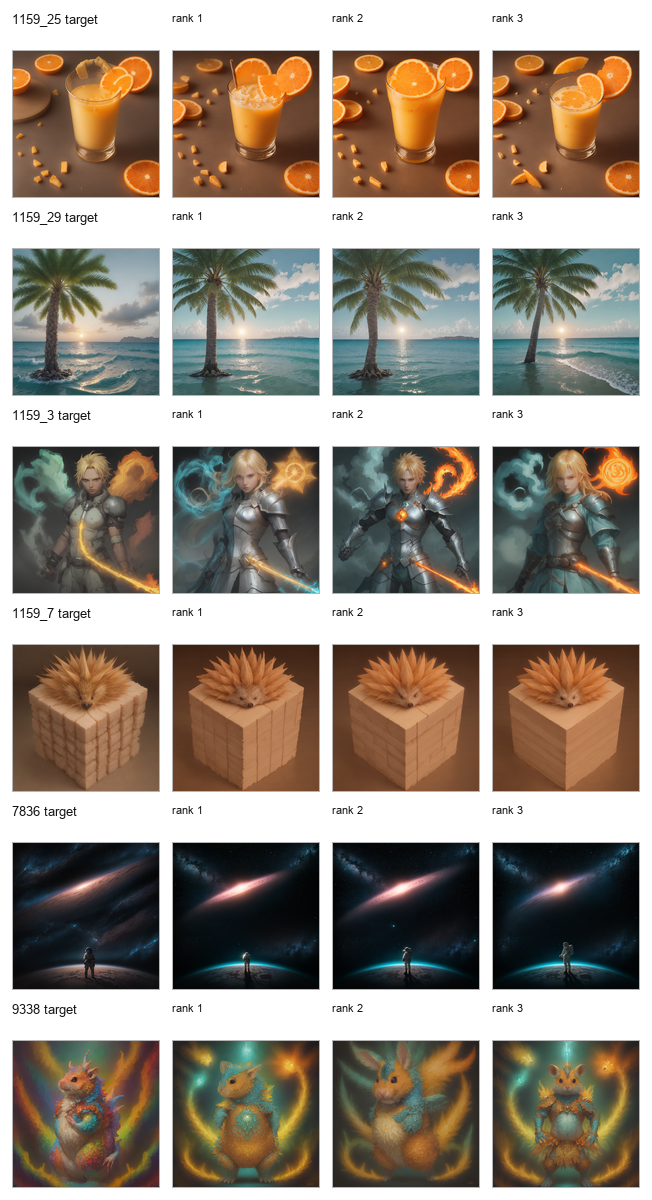
\includegraphics[height=0.86\textheight,keepaspectratio]{../imagens/figuras/final_current_top3_contact_sheet.png}
  \caption{Final selected candidates. Each row shows the target followed by the metric-ranked top-3 reconstructions.}
  \label{fig:finaltop3}
\end{figure}

\begin{table}[H]
\centering
\caption{Final top-3 candidates grouped by target image, with the renumbered source round and comparable raw score. Higher is better for Score, CLIP, and SSIM; lower is better for LPIPS and RMSE.}
\label{tab:top3}
\scriptsize
\setlength{\tabcolsep}{2.6pt}
\begin{tabular}{llrrrrrrr}
\toprule
Image & File & Rank & Round & Score & CLIP & LPIPS & RMSE & SSIM \\
\midrule
Orange juice & 1159\_25 & 1 & 20 & 0.851 & 0.951 & 0.261 & 0.111 & 0.823 \\
 & 1159\_25 & 2 & 14 & 0.850 & 0.954 & 0.263 & 0.117 & 0.827 \\
 & 1159\_25 & 3 & 14 & 0.846 & 0.946 & 0.282 & 0.109 & 0.829 \\
\midrule
Palm tree & 1159\_29 & 1 & 14 & 0.780 & 0.925 & 0.451 & 0.137 & 0.782 \\
 & 1159\_29 & 2 & 1 & 0.759 & 0.914 & 0.481 & 0.138 & 0.741 \\
 & 1159\_29 & 3 & 3 & 0.754 & 0.925 & 0.504 & 0.142 & 0.739 \\
\midrule
Anime warrior & 1159\_3 & 1 & 18 & 0.708 & 0.805 & 0.492 & 0.139 & 0.656 \\
 & 1159\_3 & 2 & 14 & 0.705 & 0.878 & 0.526 & 0.140 & 0.609 \\
 & 1159\_3 & 3 & 18 & 0.703 & 0.840 & 0.480 & 0.146 & 0.597 \\
\midrule
Hedgehog cube & 1159\_7 & 1 & 15 & 0.822 & 0.847 & 0.349 & 0.073 & 0.862 \\
 & 1159\_7 & 2 & 15 & 0.820 & 0.793 & 0.312 & 0.072 & 0.872 \\
 & 1159\_7 & 3 & 15 & 0.813 & 0.830 & 0.356 & 0.078 & 0.856 \\
\midrule
Astronaut & 7836 & 1 & 21 & 0.829 & 0.934 & 0.345 & 0.084 & 0.810 \\
 & 7836 & 2 & 20 & 0.822 & 0.917 & 0.354 & 0.087 & 0.813 \\
 & 7836 & 3 & 18 & 0.818 & 0.888 & 0.355 & 0.084 & 0.823 \\
\midrule
Fantasy hamster & 9338 & 1 & 17 & 0.743 & 0.906 & 0.494 & 0.119 & 0.679 \\
 & 9338 & 2 & 17 & 0.733 & 0.849 & 0.528 & 0.105 & 0.716 \\
 & 9338 & 3 & 21 & 0.731 & 0.851 & 0.478 & 0.115 & 0.664 \\

\end{tabular}
\end{table}

\section{Qualitative Analysis}

\paragraph{\imgpath{1159\_25.png}: orange juice.}
This was the most stable target. The final prompt family correctly captures a single glass, pale orange juice, orange slice garnish, citrus fragments, and a warm brown product-photography surface. The main residual errors are the exact garnish geometry and the amount of foam/creaminess in the juice. Removing overly descriptive terms improved realism and reduced milky artefacts.

\paragraph{\imgpath{1159\_29.png}: palm tree.}
The best candidates capture the single palm tree, turquoise water, low sun, and reflection. The model is sensitive to wave wording: strong surf terms generate waves that are too large, while compact expressions such as \emph{gentle surf and reflective foreground water} keep the water closer to the target. The remaining gap is the exact trunk placement and the amount of sunset cloud shadow.

\paragraph{\imgpath{1159\_3.png}: anime warrior.}
This target remains difficult because pose, armour reflectance, blade position, and background colour all change with small wording variations. The best candidates recover the centred blond warrior, silver armour, orange energy, and blue-green mist, but the exact blade path and face are still unstable. Lower-contrast and matte wording helped avoid overly reflective armour.

\paragraph{\imgpath{1159\_7.png}: hedgehog-cube.}
The hedgehog-cube required the most structural prompt control. Broad prompts often produced either a normal hedgehog or a decorative box. The strongest prompts explicitly describe a wooden cube body, peach-beige square sides, a hidden muzzle, and tall orange radial quills. Pixel-level metrics are strong here because the object has a compact silhouette and a uniform warm background.

\paragraph{\imgpath{7836.png}: astronaut.}
Compact space prompts worked well: a tiny astronaut at the bottom, a curved ground arc, a pale pink diagonal planetary stripe, and blue nebula haze across the image. The target is forgiving for CLIP because the concepts are common, but RMSE and SSIM reveal small layout differences in the horizon arc and diagonal stripe.

\paragraph{\imgpath{9338.png}: fantasy hamster.}
This is the most semantically fragile target. If the prompt emphasises dragon/scales too strongly, the animal becomes reptilian; if it emphasises hamster too strongly, the scale quills and rainbow aura disappear. The best prompts balance orange/teal hamster anatomy, a glowing belly patch, rainbow scale quills on the back, and a painterly aura. The remaining limitation is fine-grained control of the hybrid anatomy.

\section{Final Prompts}

Table~\ref{tab:finalprompts} lists the final top-3 prompts selected by the metric pipeline, identifying each target by its visual content and filename. The corresponding images and full metric CSV are stored in \texttt{Relatorio/dados/final\_current\_top3.csv}.

{\scriptsize
\setlength{\LTpre}{2pt}
\setlength{\LTpost}{2pt}
\setlength{\tabcolsep}{3pt}
\renewcommand{\arraystretch}{0.92}
\begin{longtable}{p{0.18\linewidth}c p{0.70\linewidth}}
\caption{Final prompts by target image content and metric rank.}
\label{tab:finalprompts}\\
\toprule
Target image & Rank & Prompt \\
\midrule
\endfirsthead
\toprule
Target image & Rank & Prompt \\
\midrule
\endhead
\bottomrule
\endfoot
\textbf{Orange juice}\\(\imgpath{1159\_25.png}) & 1 & realistic orange juice still life, single clear glass, pale orange juice without milky creaminess, orange slice on the rim, minimal citrus pieces on brown studio surface, warm realistic product photo \\
 & 2 & orange juice still life, single tall clear glass, pale orange juice, orange slice on the rim, scattered tiny citrus pieces on brown tabletop, warm realistic product photo \\
 & 3 & realistic orange juice still life, single clear glass, pale creamy orange juice, orange slice on the rim, minimal citrus pieces on brown studio surface, warm realistic product photo \\
\midrule
\textbf{Palm tree in ocean}\\(\imgpath{1159\_29.png}) & 1 & single slender palm tree rising from shallow turquoise ocean, gentle surf and reflective foreground water, low sun reflection behind the tree, shallow turquoise sea, muted colors \\
 & 2 & single slender palm tree in calm turquoise water, water fills foreground around the palm, low sun reflection behind the tree, muted colors, natural ocean photograph \\
 & 3 & single slender palm tree rising from shallow turquoise ocean, shallow surf and reflective water in foreground, low sun reflection behind the tree, soft atmospheric tropical photo \\
\midrule
\textbf{Anime warrior}\\(\imgpath{1159\_3.png}) & 1 & centered blond battle mage, light grey segmented armor, diagonal golden energy slash across front, teal ghost smoke cloud on the left, soft brushwork square crop \\
 & 2 & single blond anime warrior mage in reflective silver armor, curved amber energy blade crossing the lower body, blue green mist and orange fire clouds behind, soft brushwork, centered square composition, low contrast \\
 & 3 & single stern blond anime warrior mage, teal ghost smoke cloud on the left, orange smoke blob behind right shoulder, flat painterly anime concept art, centered square composition \\
\midrule
\textbf{Hedgehog cube}\\(\imgpath{1159\_7.png}) & 1 & small hedgehog in wooden cube, peach beige square tile sides, muzzle peeking through bristles, tall orange radial quills, flat pale top rim visible, fibrous wooden block texture, warm brown studio background, tight square crop \\
 & 2 & small hedgehog in wooden cube, peach beige square tile sides, muzzle peeking through bristles, tall orange radial quills, square wooden top plane, soft balsa wood grain, warm brown studio background, centered realistic square photo \\
 & 3 & small hedgehog in wooden cube, peach beige square tile sides, muzzle peeking through bristles, tall orange radial quills, square wooden top plane, soft balsa wood grain, warm brown studio background, tight square crop \\
\midrule
\textbf{Astronaut in space}\\(\imgpath{7836.png}) & 1 & tiny astronaut standing bottom center, thin curved ground arc reflecting pale pink light, wide pale pink diagonal planetary stripe, slanted planetary ring, subtle blue nebula clouds spread through most of the image, moody realistic space illustration \\
 & 2 & tiny astronaut standing bottom center, thin curved ground arc reflecting pale pink light, wide pale pink diagonal planetary stripe, slanted planetary ring from lower left to upper right, subtle blue nebula clouds across most of the sky, moody realistic space illustration \\
 & 3 & tiny astronaut standing bottom center, thin curved ground arc under the astronaut, wide pale pink diagonal planetary stripe, slanted planetary ring from lower left to upper right, subtle blue nebula clouds around the edges, moody realistic space illustration \\
\midrule
\textbf{Fantasy hamster}\\(\imgpath{9338.png}) & 1 & orange teal fantasy hamster with scales, single creature looking left, orange rounded snout and small ears, blue green glowing belly patch, rainbow scale quills on shoulder and back, tiny paws close to the belly, yellow orange painterly aura, storybook painterly illustration \\
 & 2 & orange teal fantasy hamster with scales, side facing orange face, small orange muzzle and black eye, blue green glowing belly patch, rainbow scale quills on shoulder and back, compact cute body, yellow orange painterly aura, vertical storybook painting \\
 & 3 & orange teal fantasy hamster with scales, single creature looking left, orange rounded snout and small ears, blue green glowing belly patch, rainbow scale quills on shoulder and back, tiny paws close to the chest, yellow orange painterly aura, storybook painterly illustration \\
\end{longtable}

}

\section{Ablation and Error Analysis}

\subsection{Metric Disagreements}

The metrics often disagreed, which is expected because each one rewards a different property. CLIP is the strongest semantic filter: it recognises that a render contains an astronaut, palm tree, or hamster-like creature even if the exact pose differs. However, CLIP can over-rank visually poor candidates when the main nouns are present. This happened frequently for \imgpath{9338.png}, where many candidates were semantically close to ``fantasy creature'' but structurally far from the target.

LPIPS was more useful for perceptual realism and local texture. It penalised incorrect object surfaces and helped distinguish the hedgehog-cube from ordinary hedgehog renders. However, LPIPS can be harsh when a target contains stylised painterly content, because small changes in brush texture alter deep features. RMSE and SSIM were useful for simple, layout-dominated images such as \imgpath{7836.png}; for the fantasy creature they were less reliable because different plausible painterly textures can have similar colour distributions but wrong anatomy.

For this reason, the final ranking never used a single metric in isolation. The internal score used normalised metric stacks, while the report exposes the raw values to keep the comparison interpretable. Visual inspection was used only as a sanity check after ranking, not as a replacement for the metric pipeline.

\subsection{Prompt Length and Token Budget}

An important negative result was that longer prompts did not consistently improve quality. The generator reacts strongly to early and concrete terms, while late descriptors often become weak style hints. Several failed prompts attempted to encode every visual detail in one sentence: material, lighting, object geometry, background, colour palette, pose, texture, and negative constraints. These prompts frequently produced clutter or shifted the main object away from the target.

The final prompt style is therefore compressed. Each prompt keeps a small number of high-value terms, usually ordered from global identity to local detail. For example, the best palm prompts begin with \emph{single slender palm tree rising from shallow turquoise ocean}; this fixes the scene before adding \emph{gentle surf} or \emph{low sun reflection}. Similarly, the hedgehog-cube prompts begin with \emph{small hedgehog in wooden cube}; the cube structure is introduced before fur, muzzle, and background. This ordering matters because it reduces ambiguity about the main object.

\subsection{Seed Sweep and Excluded Techniques}

The seed sweep runs confirmed that the same prompt can produce visibly different quality under nearby seeds. This was used only as a discovery tool: prompts that remained semantically stable across offsets were considered better candidates for fixed-seed micro-refinement, but the submitted render always uses the official seed. This was especially useful for \imgpath{9338.png}, where small stochastic changes can decide whether the model creates a mammal, a reptile, a winged creature, or a painterly mascot.

Several stronger image-generation techniques were deliberately excluded from the final render. ControlNet, image conditioning, LoRA, textual inversion, or embedding optimisation could improve structural fidelity, but they would change the task from discrete prompt recovery into conditioning or model adaptation. The final workflow only borrows their intuition indirectly: regional scoring imitates local conditioning, hard-prompt search explores discrete text alternatives, and multi-seed validation measures robustness without changing the submitted seed.

\subsection{Failure Mode Catalogue}

The most common failure modes were repeated across many prompt families. Table~\ref{tab:failures} summarises the failure, its probable cause, and the mitigation used in later rounds. The key pattern is that adding more description often fixes one attribute while breaking another. This is why the final search preferred controlled local mutations around strong anchors instead of unconstrained prompt expansion.

\begin{table}[H]
\centering
\caption{Recurring failure modes observed during prompt search.}
\label{tab:failures}
\footnotesize
\begin{tabular}{p{0.20\linewidth}p{0.34\linewidth}p{0.36\linewidth}}
\toprule
Failure mode & Typical cause & Mitigation \\
\midrule
Extra objects or clutter & prompts with too many nouns competing for attention & remove secondary nouns and keep one dominant subject phrase \\
Wrong material & generic object term dominates over material term & move material earlier, e.g. wooden cube body before fur details \\
Over-stylisation & style terms such as fantasy, dramatic, glowing, cinematic overpower geometry & keep style as the final prompt block and reduce adjectives \\
Pose drift & character prompts under-specify body orientation and energy position & add centred composition and simple directional constraints \\
Colour drift & semantically correct render uses target-incompatible palette & add one or two discriminative colour terms and use colour histogram scoring \\
Good semantic match but poor structure & CLIP ranks the object class but ignores exact layout & combine CLIP with LPIPS, SSIM, edge, and layout metrics \\
Seed-dependent success & prompt works only for one stochastic sample & use seed sweep only to discover robust prompt families \\
\bottomrule
\end{tabular}
\end{table}

The orange juice mainly suffered from colour and opacity drift. The word \emph{creamy} sometimes helped approximate the target liquid, but it also made the juice look like a milkshake. The final prompts keep the product-photography structure and use \emph{pale orange juice} rather than a long list of texture descriptors.

The palm tree mainly suffered from scale drift in the water. Words such as \emph{surf} and \emph{waves} are visually useful, but the model can interpret them as a beach scene with large waves. The final prompt uses gentler wording and avoids mentioning beach or island, because those terms often introduce land masses absent from the target.

The warrior and fantasy hamster exposed the hardest limitation of text-only inversion: the prompt must specify both object identity and exact internal structure. In these classes, failures are not just small colour differences; they are changes in anatomy, pose, or object composition. This explains why targeted search improved them more than simple prompt rewriting, but also why they remain the weakest categories.

\section{Discussion}

The most useful technical conclusion is that prompt inversion with a fixed LCM is closer to search than to normal captioning. Long descriptive prompts often performed worse because the CLIP text encoder has limited context capacity and because competing concepts interfere inside the generator. The strongest prompts usually used five to eight visual blocks: object identity, material/colour, pose/layout, background, and style.

Several attempted strategies were useful as discovery tools but not as final rendering methods. Multi-seed search helped identify robust prompt families, but the final render still uses the fixed seed. PEZ-style and hard-token search expanded the vocabulary, but the best final prompts remained human-readable. VLM-style iterative refinement was less productive than broad controlled variation because it tended to over-correct single differences and introduce new artefacts.

The biggest remaining limitation is absence of image conditioning. With text only, the model cannot be forced to preserve exact object geometry, especially for the warrior and fantasy hamster. Within the assignment constraints, the best practical improvement is not a new architecture but more targeted search around the strongest prompt families, with metric selection and visual inspection.

\subsection{Practical Lessons}

The first practical lesson is that prompt search should be organised around hypotheses, not random wording changes. When a target fails, the useful question is not only which word to add, but which visual attribute is currently wrong. For the palm tree, the relevant hypotheses were water activity, trunk placement, and sunset colour. For the hedgehog-cube, they were cube material, block separation, and whether the face should be visible. This made later rounds more productive because each group of variants tested a concrete visual assumption.

The second lesson is that shorter prompts are easier to debug. If a ten-block prompt fails, it is hard to know whether the error comes from object identity, style, material, or ordering. With compact prompts, changing one phrase has a more interpretable effect. This is why the final search often returned to simple anchors such as \emph{small hedgehog in wooden cube} or \emph{tiny astronaut standing bottom center} before adding secondary details.

The third lesson is that metrics should guide the search, but not define the entire project. Metrics are essential for screening hundreds or thousands of images, yet the final task is still visual. A metric stack can find candidates that are globally close, but it cannot fully understand whether a hamster-dragon ``feels'' like the target hybrid. The most reliable workflow was therefore automatic ranking followed by limited visual auditing of the top candidates.

The final lesson is that negative results are useful. Failed Chinese prompts, overlong prompts, highly reflective armour prompts, and aggressive surf prompts all helped define the boundaries of the generator. Each failed family removed a region of the search space and made later prompt banks smaller and more focused. This was especially important near the end, where exhaustive exploration was too expensive and targeted refinements had to be chosen carefully.

\section{Threats to Validity and Future Work}

The main threat to validity is that the ranking metrics are imperfect proxies for human visual similarity. CLIP, LPIPS, RMSE, and SSIM each capture useful information, but none of them fully represents the target image. A prompt can score well because it matches global colour and semantics while still missing a decisive local detail, such as the exact warrior blade position or the hamster's body proportions. This is why the report combines metric tables with qualitative analysis.

A second threat is generator stochasticity. Although the final seed is fixed, prompt quality is still partly tied to how the model interprets a text sequence under that seed. A prompt that is robust under nearby seeds is more trustworthy, but the assignment requires the filename seed, so robustness cannot replace the final fixed-seed evaluation. Future work could define a robustness-aware objective that still ranks candidates primarily by the official seed but penalises prompts that collapse under small seed offsets.

A third limitation is the absence of local controllability. Text-only prompting has no direct way to pin a palm trunk to an exact pixel location, force a 5x5x5 cube structure, or preserve a precise diagonal energy blade. Future work inside the same discrete-prompt constraint would focus on better prompt search policies: adaptive sampling, automatic term ablation, and learned proposals from the best/worst candidates in each round.

If the task allowed additional conditioning, the most effective extensions would likely be ControlNet-style structure guidance or textual inversion. However, those approaches would change the nature of the assignment. For the present setting, the most appropriate future improvement is a stronger evaluator that explicitly detects target-specific failures, such as multiple subjects, missing teal belly, non-cubic hedgehog body, or excessive wave height in the palm image.

\enlargethispage{3\baselineskip}
\section{Conclusion}

The final system treats image-to-prompt inversion as a constrained search problem rather than as ordinary image captioning. Across 23 experimental rounds, the most reliable workflow was to generate structured prompt families, render them with the official fixed seed, evaluate them with complementary metrics, and then use visual inspection only as a limited sanity check. This produced the strongest results on targets with stable semantics or compact layouts, especially the orange juice, palm tree, astronaut, and hedgehog-cube.

The harder cases, particularly the warrior and fantasy hamster, show the main limitation of text-only inversion. Without image conditioning or model adaptation, the prompt cannot force exact pose, local geometry, or hybrid anatomy; small wording changes can regenerate the entire composition. Even so, the final fixed-seed top-3 set is traceable to the round history, reproducible from plain text prompts, and supported by a cross-round metric audit. The main conclusion is therefore practical: under the assignment constraints, carefully controlled prompt search with multi-metric ranking is more effective than longer descriptions or purely iterative prompt rewriting. Just as important, the project leaves a reusable workflow in which prompt banks, round summaries, retained images, and consolidated CSV files make each final choice auditable. The strongest outcome is therefore not only the submitted prompts, but a reproducible search procedure that another user can rerun, inspect, and extend under the same fixed-generation constraints.

\begingroup
\footnotesize

\section*{Tools and External Components}

The implementation used \modelname, \texttt{diffusers}, \texttt{transformers}, \clipmodel, LPIPS AlexNet, PyTorch, Pillow, and custom prompt-search scripts. Codex was used as a programming assistant to generate scripts, inspect outputs, and help design prompt-search strategies. In the VLM phase, the gpt 5.5 model was used via Codex for prompt refinement, serving as a cost-free alternative to avoid per-request fees on OpenRouter. Final ranking was performed through rendered images and image metrics.

\section*{Repository and Submission Notes}

The project repository is organised so that the report can be read independently from the exploratory runs while the code still preserves the experimental workflow. The repository is structured as follows: \texttt{relatorio/} containing the final PDF report, complete LaTeX source, figures, and data; \texttt{Rondas/} containing the history of the 23 experimental rounds, where each round is self-contained with its own code (\texttt{codigo}), notebooks (\texttt{notebook}), and results (\texttt{resultados}); \texttt{targets/} containing the six target images; and \texttt{requirements.txt} containing the Python dependencies. Large obsolete intermediate files were removed to keep the submission package compact.

The most important result file is \texttt{Relatorio/dados/final\_current\_top3.csv}. It maps each target and rank to the selected prompt, rendered image path, CLIP, LPIPS, RMSE, SSIM, and source run. The contact sheet used in the report was generated from the same CSV, so the CSV is the authoritative link between prompts, images, and reported metrics.

The README should keep reproduction minimal: install dependencies, load \modelname, run the final fixed-seed or top-k validation command, and compare the generated CSV with \texttt{final\_current\_top3.csv}. It should also state that offline execution requires the model checkpoint to already exist in the Hugging Face cache. Full historical reproduction is not necessary for grading, because the selected prompts, images, metrics, and scripts are enough to validate the final approach.

Large obsolete render folders may be excluded if storage is a concern. The compact artefacts are more important than every failed image because they preserve the relevant evidence: prompt text, metric values, target identity, rank, output path, and source information. A useful final sanity check is to verify that every path referenced by \texttt{final\_current\_top3.csv} exists and that the contact sheet can be regenerated from it.

\endgroup

\begingroup
\footnotesize
\begin{thebibliography}{6}
\bibitem{lcm} Luo, S., Tan, Y., Huang, L., Li, J., Zhao, H.: Latent Consistency Models: Synthesizing High-Resolution Images with Few-Step Inference. arXiv:2310.04378 (2023)
\bibitem{sd} Rombach, R., Blattmann, A., Lorenz, D., Esser, P., Ommer, B.: High-Resolution Image Synthesis with Latent Diffusion Models. CVPR (2022)
\bibitem{clip} Radford, A., et al.: Learning Transferable Visual Models From Natural Language Supervision. ICML (2021)
\bibitem{lpips} Zhang, R., Isola, P., Efros, A.A., Shechtman, E., Wang, O.: The Unreasonable Effectiveness of Deep Features as a Perceptual Metric. CVPR (2018)
\bibitem{pez} Wen, Y., et al.: Hard Prompts Made Easy: Gradient-Based Discrete Optimization for Prompt Tuning and Discovery. NeurIPS (2023)
\bibitem{prompting} Mahajan, S., Rahman, T., Yi, K.M., Sigal, L.: Prompting Hard or Hardly Prompting: Prompt Inversion for Text-to-Image Diffusion Models. CVPR (2024)
\end{thebibliography}
\endgroup

\end{document}
